%% This is file `elsarticle-template-1-num.tex',
%%
%% Copyright 2009 Elsevier Ltd
%%
%% This file is part of the 'Elsarticle Bundle'.
%% ---------------------------------------------
%%
%% It may be distributed under the conditions of the LaTeX Project Public
%% License, either version 1.2 of this license or (at your option) any
%% later version.  The latest version of this license is in
%%    http://www.latex-project.org/lppl.txt
%% and version 1.2 or later is part of all distributions of LaTeX
%% version 1999/12/01 or later.
%%
%% The list of all files belonging to the 'Elsarticle Bundle' is
%% given in the file `manifest.txt'.
%%
%% Template article for Elsevier's document class `elsarticle'
%% with numbered style bibliographic references
%%
%% $Id: elsarticle-template-1-num.tex 149 2009-10-08 05:01:15Z rishi $
%% $URL: http://lenova.river-valley.com/svn/elsbst/trunk/elsarticle-template-1-num.tex $
%%
\documentclass[preprint,12pt]{elsarticle}

%% Use the option review to obtain double line spacing
%% \documentclass[preprint,review,12pt]{elsarticle}

%% Use the options 1p,twocolumn; 3p; 3p,twocolumn; 5p; or 5p,twocolumn
%% for a journal layout:
%% \documentclass[final,1p,times]{elsarticle}
%% \documentclass[final,1p,times,twocolumn]{elsarticle}
%% \documentclass[final,3p,times]{elsarticle}
%% \documentclass[final,3p,times,twocolumn]{elsarticle}
%% \documentclass[final,5p,times]{elsarticle}
%% \documentclass[final,5p,times,twocolumn]{elsarticle}

%% if you use PostScript figures in your article
%% use the graphics package for simple commands
%% \usepackage{graphics}
%% or use the graphicx package for more complicated commands
%% \usepackage{graphicx}
%% or use the epsfig package if you prefer to use the old commands
%% \usepackage{epsfig}

%% The amssymb package provides various useful mathematical symbols
\usepackage{amssymb}
%% The amsthm package provides extended theorem environments
%% \usepackage{amsthm}

\usepackage{siunitx}
\usepackage[utf8]{inputenc}
\usepackage[T1]{fontenc}
\usepackage{todo}
\usepackage{textcomp}

%% The lineno packages adds line numbers. Start line numbering with
%% \begin{linenumbers}, end it with \end{linenumbers}. Or switch it on
%% for the whole article with \linenumbers after \end{frontmatter}.
\usepackage{lineno}

%% natbib.sty is loaded by default. However, natbib options can be
%% provided with \biboptions{...} command. Following options are
%% valid:

%%   round  -  round parentheses are used (default)
%%   square -  square brackets are used   [option]
%%   curly  -  curly braces are used      {option}
%%   angle  -  angle brackets are used    <option>
%%   semicolon  -  multiple citations separated by semi-colon
%%   colon  - same as semicolon, an earlier confusion
%%   comma  -  separated by comma
%%   numbers-  selects numerical citations
%%   super  -  numerical citations as superscripts
%%   sort   -  sorts multiple citations according to order in ref. list
%%   sort&compress   -  like sort, but also compresses numerical citations
%%   compress - compresses without sorting
%%
\biboptions{comma,round}

% \biboptions{}
\journal{Journal of Chromatography A}

\begin{document}

\newcommand{\oneD}{\textsuperscript{1}D\xspace}
\newcommand{\twoD}{\textsuperscript{2}D\xspace}

\begin{frontmatter}

%% Title, authors and addresses

%% use the tnoteref command within \title for footnotes;
%% use the tnotetext command for the associated footnote;
%% use the fnref command within \author or \address for footnotes;
%% use the fntext command for the associated footnote;
%% use the corref command within \author for corresponding author footnotes;
%% use the cortext command for the associated footnote;
%% use the ead command for the email address,
%% and the form \ead[url] for the home page:
%%
%% \title{Title\tnoteref{label1}}
%% \tnotetext[label1]{}
%% \author{Name\corref{cor1}\fnref{label2}}
%% \ead{email address}
%% \ead[url]{home page}
%% \fntext[label2]{}
%% \cortext[cor1]{}
%% \address{Address\fnref{label3}}
%% \fntext[label3]{}

\title{Determination of polycyclic aromatic hydrocarbons and fatty acid methyl esters in diesel fuel by comprehensively coupled (supercritical fluid \(\times\) gas) chromatography}

%% use optional labels to link authors explicitly to addresses:
%% \author[label1,label2]{<author name>}
%% \address[label1]{<address>}
%% \address[label2]{<address>}

\author{Daniel Malan}
\address{Department of Chemistry, University of Pretoria}
\ead{niel.malan@tuks.co.za}


\author{Egmont Rohwer\corref{cor1}}
\address{Department of Chemistry, University of Pretoria}
\ead{egmont.rohwer@up.ac.za}
\cortext[cor1]{Corresponding author}

\begin{abstract}
%% Text of abstract



\end{abstract}

\begin{keyword}
supercritical fluid chromatography \sep diesel \sep fatty acid methyl esters \sep polycyclic aromatic hydrocarbons \sep biodiesel

%% keywords here, in the form: keyword \sep keyword
%% MSC codes here, in the form: \MSC code \sep code
%% or \MSC[2008] code \sep code (2000 is the default)

\end{keyword}

\end{frontmatter}

%%
%% Start line numbering here if you want
%%
\linenumbers

%% main text
\section{Introduction}
\label{S:1}

Fuel for compression-ignition engines (diesel fuel) was traditionally obtained
from petroleum sources. Today these traditional fuels are being blended with and
replaced by diesel fuel from biological sources. To be sold on the open market,
these fuels must comply with certain technical requirements, set by standards
organizations such as ASTM and CEN. Because of the complexity of diesel fuel
obtained from petroleum sources (petrodiesel) the chemical composition of the
fuel is in general not prescribed. Instead, a compliant fuel must pass certain
distillation tests. There are two exceptions: the amount of polycyclic
aromatic hydrocarbons (PAHs) and fatty acid methyl esters (FAMEs) are subject to
upper limits.

PAHs are natural constituents of petrodiesel. They are noxious pollutants, and
therefore regulators try to reduce the exposure of humans to PAHs by limiting
their emission into the environment. Since a major source of PAH emissions is
internal combustion engines, one way to limit emissions is to limit the amount
in diesel fuels. A full discussion on PAH sources is beyond the scope of this paper. 

FAMEs are not found in petroleum but are blended with petrodiesel. FAMEs are
usually obtained by the transesterification of plant oils with methanol. The
resulting product can be used as a diesel fuel and is called biodiesel.  The
primary benefit of the blending of FAMEs is that it lowers the carbon footprint
of the fuel, but it can also improve the lubricity of high-paraffinic diesel
\citep{Rodriguez-Fernandez2019}. Diesel for sale in the Eurpean Union can
contain up to \SI{7}{\percent} FAMEs. Any concentration of biodiesel makes a
diesel fuel but, higher concentrations are regulated as blends.

The amount of PAHs in diesel can be determined by a fluorescent indicator
absorption (FIA) test (ASTM D1319, \citep{Knight1956}), but this method is
labour-intensive. Another method is a liquid chromatography method (EN
12916:2006) with refractive index detection, and the method prescribed by ASTM
D2425 requires a mass spectrometer. The method ASTM D5168 is a supercritical
fluid chromatography (SFC) method with flame ionization detection (FID). Because
the FID responds to number of carbon and has a large dynamic range atoms in the
sample FID methods are preferable for quantification.

The prescribed methods for determining FAMEs in diesel is an infra-red
absorption method, ASTM D7806-12. This method is liable to interference from FAMEs
degradation products that might accumulate during storage \citep{Pinho2014}.

The SFC-FID method ASTM 5186-19 claims that FAMEs interfere with the method.
\citet{Weber2016} claims that FAMEs `foul' the column. This is contrary to
experience: FAMEs do elute from silica columns with neat CO\textsubscript{2} as
mobile phase \citep{Smith2001}. But the capacity factors (\(k'\) values ) of the
PAHs are less than \num{0.05}, while the capacity factors of the FAMEs are
greater than \num{0.8}\todo{Use k' values from own experiments}. If a number of
determinations of PAHs in FAME-containing diesel fuel are done in sequence
without allowing the FAMEs to elute, the FAMEs will start eluting during the PAH
determination and cause interference. To address this problem The California Air
Resources Board (ARB) has published a standard operating procedure (SOP)
\citep{ARB2017} based on a publication by \citet{Diehl2007} that combines the
determination of PAHs with FAMEs. In this procedure SFC-FID is used to determine
the PAHs, and then the column is back-flushed to determine total FAMEs. This
solves the problem of FAMEs interfering with the PAHs determination and
simultaneously quantifies the FAMEs.

The information produced by this method is the total amount of FAMEs and the
total amounts of mono-, di-, and tri+ aromatics. This information suffices for
monitoring compliance, but extending the method by comprehensively coupling a
fast gas chromatograph (GC) to the SFC provides a richly patterned chromatogram
that can help solve process control and supply chain problems. The orthogonality
of SFC and GC is high: on SFC with bare silica as a stationary phase and neat
carbon dioxide as a mobile phase PAHs are separated according to the number of
rings in their structure, and the FAMEs are separated according to the number of
double bonds, whereas all GC separations are primarily according to volatility.
Therefore determining PAHs and FAMEs make an ideal combination for
comprehensively coupled (supercritical fluid \(\times\) gas) chromatography.
If --- using the ARB SOP as a basis --- the FAMEs are not back-flushed but all
the compounds are allowed to elute,  and the SFC is comprehensively coupled to
gas chromatography (GC), the \textsuperscript{1}D (SFC) dimension will separate
the PAHs into their classes, and the FAMES according to the number of double
bonds. The \textsuperscript{2}D (GC) separation will separate the compounds in
each PAH and FAME class further, according to their volatility. The resulting
chromatogram contains patterns that are rich in information.

% These people \citep{Paproski2006} do it fast.

% \citep{Squicciarini1996} did it using a silver column.

%\begin{itemize}
%%\item Bullet point one
%\item Bullet point two
%\end{itemize}

%\begin{enumerate}
%\item Numbered list item one
%\item Numbered list item two
%\end{enumerate}

%\subsection{Subsection One}

%\begin{table}[h]
%\centering
%\begin{tabular}{l l l}
%\hline
%\textbf{Treatments} & \textbf{Response 1} & \textbf{Response 2}\\
%\hline
%Treatment 1 & 0.0003262 & 0.562 \\
%Treatment 2 & 0.0015681 & 0.910 \\
%Treatment 3 & 0.0009271 & 0.296 \\
%\hline
%\end{tabular}
%\caption{Table caption}
%\end{table}

%\subsection{Subsection Two}

%Donec eget ligula venenatis est posuere eleifend in sit amet diam. Vestibulum sollicitudin mauris ac augue blandit ultricies. Nulla facilisi. Etiam ut turpis nunc. Praesent leo orci, tincidunt vitae feugiat eu, feugiat a massa. Duis mauris ipsum, tempor vel condimentum nec, suscipit non mi. Fusce quis urna dictum felis posuere sagittis ac sit amet erat. In in ultrices lectus. Nulla vitae ipsum lectus, a gravida erat. Etiam quam nisl, blandit ut porta in, accumsan a nibh. Phasellus sodales euismod dolor sit amet elementum. Phasellus varius placerat erat, nec gravida libero pellentesque id. Fusce nisi ante, euismod nec cursus at, suscipit a enim. Nulla facilisi.

%\begin{figure}[h]
%\centering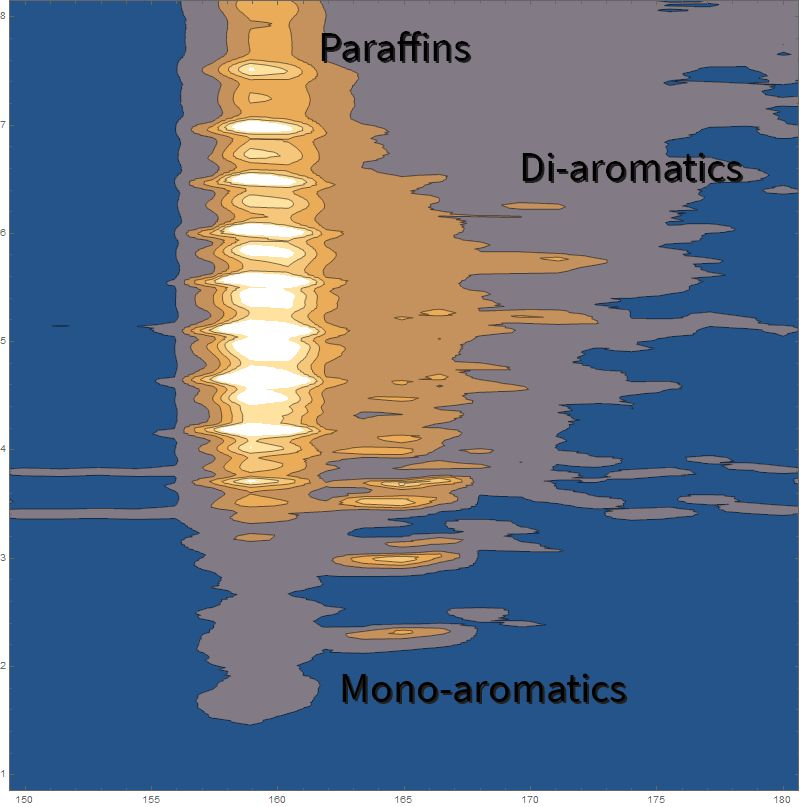
\includegraphics[width=0.4\linewidth]{Aromatics}
%\caption{Figure caption}
%\end{figure}

%Integer risus dui, condimentum et gravida vitae, adipiscing et enim. Aliquam erat volutpat. Pellentesque diam sapien, egestas eget gravida ut, tempor eu nulla. Vestibulum mollis pretium lacus eget venenatis. Fusce gravida nisl quis est molestie eu luctus ipsum pretium. Maecenas non eros lorem, vel adipiscing odio. Etiam dolor risus, mattis in pellentesque id, pellentesque eu nibh. Mauris nec ante at orci ultricies placerat ac non massa. Aenean imperdiet, ante eu sollicitudin vestibulum, dolor felis dapibus arcu, sit amet fermentum urna nibh sit amet mauris. Suspendisse adipiscing mollis dolor quis lobortis.

%\begin{equation}
%\label{eq:emc}
%e = mc^2
%\end{equation}

\section{Material and methods}


    
\section{Results}

Figure \ref{fig:Aromatics} shows some results.

\begin{figure}[h]
\centering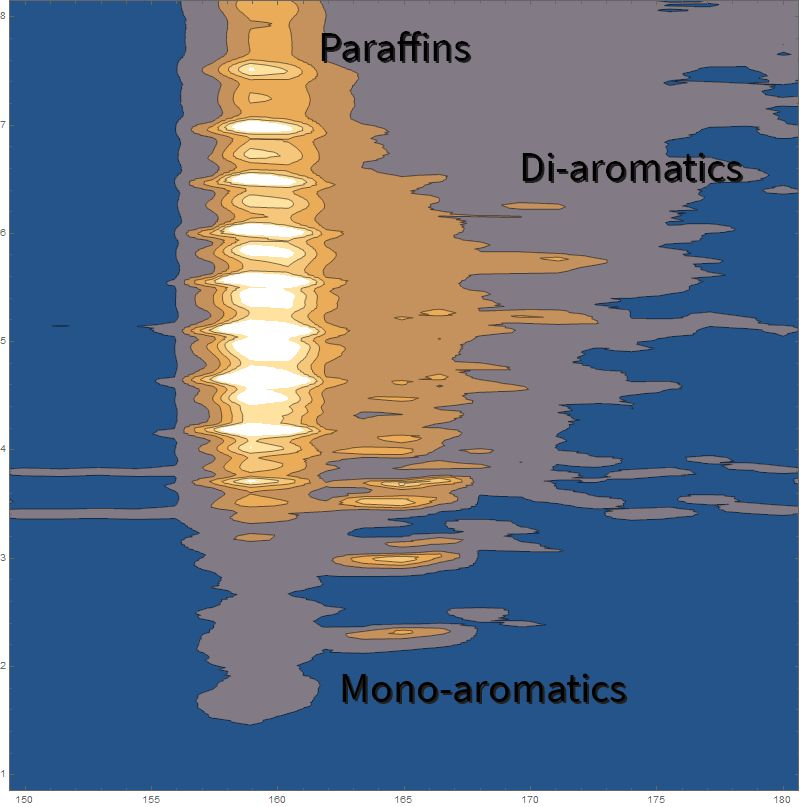
\includegraphics[width=0.4\linewidth]{Aromatics}
\caption{\label{fig:Aromatics}. A contour plot of an SFCxGC chromatogram, showing the hydrocarbons in detail}
\end{figure}

    
\section{Discussion}

    
\section{Conclusion}

\section*{ Acknowledgements}

\todos{}

%% The Appendices part is started with the command \appendix;
%% appendix sections are then done as normal sections
%% \appendix

%% \section{}
%% \label{}

%% References 
%%
%% Following citation commands can be used in the body text:
%% Usage of \cite is as follows:
%%   \cite{key}          ==>>  [#]
%%   \cite[chap. 2]{key} ==>>  [#, chap. 2]
%%   \citet{key}         ==>>  Author [#]

%% References with bibTeX database:

\bibliographystyle{model1-num-names}
\bibliography{DieselPAHFAMES}

%% Authors are advised to submit their bibtex database files. They are
%% requested to list a bibtex style file in the manuscript if they do
%% not want to use model1-num-names.bst.

%% References without bibTeX database:

% \begin{thebibliography}{00}

%% \bibitem must have the following form:
%%   \bibitem{key}...
%%

% \bibitem{}

% \end{thebibliography}


\end{document}

%%
%% End of file `elsarticle-template-1-num.tex'.
